\subsection{Међурепрезентација високог нивоа (МВН) - High-Level Intermediate Representation (HIR)}

\subsubsection{Конструкција}

Обрадом проширеног облика апстрактног синтаксног стабла настаје међурепрезентација високог нивоа.
Процес обраде се назива снижавање (\verb|lowering|). Неке синтаксне форме бивају поједностављене.
Заграде се уклањају јер структура стабла експлицитно одређује редослед операција. \verb|For| петље 
се конвертују у \verb|while(let)| петље \ref{lst:hir_iter}. Израз \verb|if let| се преводи 
у \verb|match| израз. Израз \verb|impl| у параметрима функције се конвертује у генерички аргумент.
Поједностављење је начин да се заобиђу гранични случајеви и смањи количина кода која је потребна 
да се изворни код анализира.

\begin{listing}[H]
\begin{minted}{rust}
// Pre
for elem in vec {
    process(elem);
}
// Posle
let mut iterator = vec.into_iter();
while let Some(elem) = iterator.next() {
    process(elem);
}
\end{minted}
\caption{"for" петља пре и након поједностављења}
\label{lst:hir_iter}
\end{listing}

\verb|Crate| је поново чвор највишег нова али за разлику \verb|Crate|-а апстрактног синтаксног стабла који садржи
само податке о коренском модулу, \verb|Crate| високе међурепрезентације складишти садржај целокупног пакета.
Изворни код који се не користи нити имплицитно нити екплицитно није постојан унутар овог погледа. Значај 
ове особине се највише испољава приликом употребе екстерних библиотека, где је уобичајно користити само 
део функционалности.

\subsubsection{Систем упита}

\verb|HIR| је најкоришћенији облик изворног кода у \verb|rustc| \verb|frontend|-у. Такође је први облик који 
користи систем упита (\verb|query|) и од изузетне је важности приликом инкременталног компајлирања.
Из перспективе компајлера знање у вези \verb|Crate|-а је база података, док су упити начин на који 
се добављају подаци. Наиме кључна разлика између стандардне базе података и "базе података" компајлера
то што "база података" компајлера почиње празна и пуни се када се упити изврше. То значи да упит мора 
да зна како да израчуна излаз у случају да резултат не постоји у "бази података". "База података" компајлера 
се назива контекст упита.

Упит се идентификује помоћу имена. Кључ специфицира који податак треба да се добави и тај податак 
мора да поседује повратни тип. Провајдер је функција која специфицира како се рачуна резултат уколико није 
претходно израчунат. Есенцијално, упит је функција која мапира кључ на резултат. 
Повратне вредности упита се кеширају. Повратна вредност било којег суксесивног упита са истим параметарима резултоваће 
копији већ израчунате вредности унутар кеша. Оваква техника кеширања резултата се назива мемоизација.
Кеширање је неопходно да би систем упита био ефикасан. Без њега исте калкулације би се понављале произвољан број пута.

Да би овај систем функционисао на претходно описан начин уводе се поједина правила. Кључ и резултат 
морају бити непроменљиве вредности. Провајдер мора бити детерминистичка функција, тј. упит за исти кључ
увек враћа исту вредност. Једини параметри упита јесу кључ и констекст компајлирања (база података).
Мемоизација је један од главних разлога за ова правила. Уколико би провајдер могао да врати недетерминистички резултат,
тачност кеширањог резултата не би могла бити загарантована.

Позиви упита морају да креирају дирекциони ациклични граф. Пошто су провајдери само обичне функције лако је претворити 
ациклични граф у циклични додавањем функције која креира циклус. Раније је \verb|rustc| компајлер имао подршку 
за прекидање циклуса и наставком рада, али теоретски такво извршавање није детерминистичко и није засигурно да би 
инкрементално компајлирање радило. Данас, систем упита пријављује грешку да је пронађен циклус
и не наставља са компајлирањем.

Резултати упита могу бити украдени, тј. резултат се налази унутар структуре \verb|Steal<t>| и очекује се да ће се власништво 
пренети ка неком другом контексту у неком тренутку. Ова техника се примарно користи због перформанси, 
јер су неке вредности скупе за клонирање. Овај поступак не наноси штету у контексту инкременталног компајлирања јер се пре 
преноса власнишва извршавају сви упити који би могли да потраже овај резултат. Са обзиром да се упити који траже резултат 
морају навести мануелно, простор за грешку је велики. Уколико је украдени резултат потражен од неког упита након што је пренето власништво
компајлер пријављује грешку, осигуравајући безбедно стање.

\subsubsection{Инкрементално компајлирање}

Инкрементално компаљирање се ослања на структуру дирекционог ацикличног графа кроз "\verb|try|-\verb|mark|-\verb|green|" алгоритам.
Овај алгоритам потиче од "\verb|red|-\verb|green|" алгоритма. Идеја је да након сваког упита се сачува резултат упита али и дирекциони 
ациклични граф тог упита тј. резултате упита које је родитељски упит позвао. Приликом суксесивног покретања компајлера потеницјално 
је могуће искористити резултат неких упита из претходне компилације. Ово се постриже додељивањем боје сваком упиту. Ако се резултат 
упита променио у односу на претходни пут, упит постаје црвен. Уколико је резултат исти као и претходни пут, упит постаје зелен. 
Из овога произилазе два нова правила. Ако су сви улази у упит исти, онда ће и резултат упита бити исти. Овим се спашава значајно време 
које би се иначе потрошило на читање и десеријализовање података са диска. Насупрот овог правила, ако се улаз у упит променио, 
а и даље је вратио исти резултат, упит се боји у зелено и заобилази се понављање овог упита.

Алгоритам "\verb|try|-\verb|mark|-\verb|green|" ради на следећи начин. Проверава да ли је упит извршен у претходној компилацији. Ако 
није, упит се евалуира и боји црвеном. Ако јесте, учитавају се сва деца (зависности) тог упита. За сваку зависност упита рекурзивно 
евалуирати боју истим редоследом као и у претходној компилацији. Уколико су све зависности зелене онда је и родитељски упит зелен.
Ако је било који чвор у овом процесу црвен, родитељски чвор је прљав. Извршавају се све зависности родитељског упита, а потом 
пореди хеш резултата са хеш-ом претходног резултата. Ако се хеш није променио родитељски упит постаје зелен, у супротном црвен.

Лажно позитивне вредности су проблем приликом употребе оваквог алгоритма. Претпоставља се да упит "одреди знак" постоји и да су 
улази почетне и наредне компилације у овај упит редом бројеви 500 и 1000. Иако је очигледно да се знак није променио, компајлер 
мора бити конзервативан и поново евалуаирати резултат овог упита.

Када компајлер престане са радом, све евалуиране вредности у меморији бивају уништене. Стога резултати упита морају да се чувају 
на диску. Ово доводи до нових проблема који се морају решити. Резултати на диску нису одмах спремни за поређење. Идентификатори 
чворова графа између компилација су потенцијално померени (\verb|NodeId|, \verb|DefId|). Перзистирање на диск има своју цену и 
није смислено сваку ситну информацију чувати на диску. 

Уколико се код није мењао и редослед дефиниција/имплементација у коду остао исти генерисани 
идентификатори остају исти, али уколико се било шта померило не постоји гаранција да је и даље тако. Овај проблем се решава 
увођењем стабилних форми идентификатора. За најбитнији случај \verb|DefId| стабилна замена је \verb|DefPath|. \verb|DefPath| није нумерички 
и ослања се на путању као што је \verb|std::collections::HashMap|, чиме није афектован нерелевантним променама у изворном коду. 
\verb|DefPathHash| је 128 битна репрезентација \verb|DefPath|. Практично гледано, обе репрезентације садрже исту информацију па се 
\verb|DefPathHash| чешће користи јер је лакши за употребу. Приликом десеријализације резултата \verb|DefPathHash| се мапира на 
\verb|DefId| из тренутне компилације. \verb|HirId| је идентификатор компоненти високе репрезентације које немају \verb|DefId|. 
\verb|HirId| је спој \verb|DefPath| и \verb|LocalId|. \verb|LocalId| идентификује израз унутар неке ставке кода, на пример 
дефиниција варијабле унутар функције.

Приликом извршавања "\verb|try|-\verb|mark|-\verb|green|" алгоритма често се пореди резултат упита тренутне компилације у односу 
на резултат упита у претходној компилацији. Десеријализација резултата са диска је скупа операција, а резултат тренутног упита је 
већ срачунат и може да се користи. Компајлер превазилази овај проблем употребом отисака приста (\verb|fingerprint|). Отисак прста 
је 128 битни хеш резултата упита. Јефтино је учитати целокупну мапу отисака прстију приликом учитавања дирекционог ацикличног графа 
и поређење се своди на јефтино упоређивање резултата из мапе. Вероватноћа да се колизија хеш вредности догоди је изузетно мала 
јер се користи квалитетан хеш. Наиме употреба квалитетног хеша доводи да у неким случајевима инкрементална компилација бива 
спорија од неинкременталне услед времена проведеног у рачунању хеш вредности. Отисци прстију се користе приликом корелације 
између чвора претходног и тренутног дирекционог ацикличног графа, тако што се отисак прста рачуна над кључем упита.

Дешава се да неки чворови између две компилације не буду евалуирани јер су чворови само зависности родитеља који је обојен 
зеленом. Пратећи претходно описан алгоритам добило би се да нови дирекциони ациклични граф не садржи више ове зависности. Због 
тога се примењује промоција кеша. Пре него што се резултат инкременталне компилације пребаци на диск, извршиће се пролазак 
кроз све зависоности сваког зеленог чвора и постараће се да су учитани у меморију. На овај начин зависности које тренутно 
нису можда неопходне могу бити искоришћене у будућим компилацијама. 

Упити могу да садрже модификаторе који утичу на то како се систем упита опходи према упиту приликом инкременталне компилације.
Модификатор \verb|eval_always| означава да упити никада неће бити зелен и прескаче се приликом "\verb|try|-\verb|mark|-\verb|green|".
Овај модификатор је користан у случају да упит чита вредност из неког фајла или глобалног стања где може доћи до мутација. Такође неки 
упити зависе од целокупног изворног кода и нема потребе покушавати кеширати резултат јер ће увек боја бити црвена. Модификатор 
\verb|no_hash| означава да за упит никада неће бити рачунат отисак прста. Из овога следи да сваки упит који зависи од \verb|no_hash|
упита мора бити рекалкулисан. Овај модификатор је користан у случају када би се отисак прста рачунао над великим и комплексним 
вредностима где би овај поступак трајао дуго. Такође за функције које су веома осетљиве на промене упита (а * б * ц), промена 
улаза ће скоро увек резултовати црвеној боји чвора. Модификатор \verb|cache_on_disk_if| одређује да ли ће резултат упита бити 
сачуван на диску. 

Модификатори \verb|eval_always| и \verb|no_hash| могу бити заједно коришћени у шаблону који се назива пројекционим упити. Постоје упити који захтевају 
целокупан улаз компајлера (индексиран \verb|HIR|). Овакви упити се често моделују тако што се велики упит макира са \verb|eval_always|
да би се сачувало време. Зависности упита (пројекције) су упити које засебно могу бити обојене црвено или зелено. Тиме се омогућава 
да неке пројекције буду црвене и евалуирана поново док остале зелене пројекције могу да искористе претходни резултат.

\begin{listing}[H]
\begin{center}
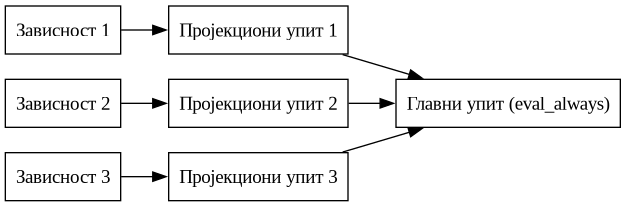
\includegraphics[width=4in, height=1.4in]{assets/images/projection_query.png}
\end{center}
\caption{Употреба "eval\_always" модификатора у пројекционом шаблону}
\label{lst:projection_query}
\end{listing}